%
% 6.006 problem set 3
%
\documentclass[12pt,twoside]{article}

\input{../macros}

\usepackage{amsmath}
\usepackage{url}
\usepackage{mdwlist}
\usepackage{graphicx}
\usepackage{clrscode3e}
\usepackage{listings}
\usepackage{tikz}
\usetikzlibrary{arrows}
\usetikzlibrary{matrix}
\usetikzlibrary{positioning}
\usetikzlibrary{shapes.geometric}
\usetikzlibrary{shapes.misc}
\usetikzlibrary{trees}

\setlength{\oddsidemargin}{0pt}
\setlength{\evensidemargin}{0pt}
\setlength{\textwidth}{6.5in}
\setlength{\topmargin}{0in}
\setlength{\textheight}{8.5in}

% Fill these in!
\newcommand{\theproblemsetnum}{3}
\newcommand{\releasedate}{September 29, 2011}
\newcommand{\partaduedate}{Thursday, October 6}
\newcommand{\tabUnit}{3ex}
\newcommand{\tabT}{\hspace*{\tabUnit}}

\begin{document}

\handout{Problem Set \theproblemsetnum}{\releasedate}

\newcommand{\solution}[1]{
  \par\medskip
  \textbf{Solution:} #1
}
%\renewcommand{\solution}[1]{ }

\textbf{Both theory and programming questions} are due {\bf \partaduedate} at
{\bf 11:59PM}.
%
Please download the .zip archive for this problem set, and refer to the
\texttt{README.txt} file for instructions on preparing your solutions.

We will provide the solutions to the problem set 10 hours after the problem set
is due, which you will use to find any errors in the proof that you submitted.
You will need to submit a critique of your solutions by \textbf{Friday,
October 7th, 11:59PM}. Your grade will be based on both your solutions and
your critique of the solutions.

\medskip

\hrulefill

\begin{problems}

\problem \points{45} \textbf{Range Queries}

Microware is preparing to launch a new database product, NoSQL Server, aimed at
the real-time analytics market. Web application analytics record information
(e.g., the times when users visit the site, or how much does it take the
server to produce a HTTP response), and can display the information using
a Pretty Graph\texttrademark\footnote{U.S. patent pending, no. 9,999,999}, so
that CTOs can claim that they're using data to back their decisions.

NoSQL Server databases will support a special kind of index, called a  
\textit{range index}, to speed up the operations needed to build a Pretty
Graph\texttrademark{} out of data. Microware has interviewed you during the fall
Career Fair, and immediately hired you as a consultant and asked you to help the
NoSQL Server team design the range index.

The range index must support fast (sub-linear) insertions, to keep up with Web
application traffic. The first step in the Pretty Graph\texttrademark{}
algorithm is finding the minimum and maximum values to be plotted, to set up the
graph's horizontal axis. So the range index must also be able to compute the
minimum and maximum over all keys quickly (in sub-linear time).

\begin{problemparts}
\problempart \points{1} Given the constraints above, what data structure covered
in 6.006 lectures should be used for the range index? Microware engineers need
to implement range indexes, so choose the simplest data struture that meets the
requirements.
\begin{enumerate}
  \item Min-Heap
  \item Max-Heap
  \item Binary Search Tree (BST)
  \item AVL Trees 
  \item B-Trees
\end{enumerate}
\solution {
  AVL trees are the only data structure that supports sub-linear
  insertions, as well as sub-linear minimum and maximum queries.
}

\problempart \points{1} How much time will it take to insert a key in the range
index?
\begin{enumerate}
  \item $O(1)$
  \item $O(\log(\log N))$
  \item $O(\log N)$
  \item $O(\log^2 N)$
  \item $O(\sqrt{N})$
\end{enumerate}
\solution {
  Inserting a node in an AVL tree takes $O(\log N)$ time. See the lecture
  notes on AVL trees.
}

\problempart \points{1} How much time will it take to find the minimum key in
the range index?
\begin{enumerate}
  \item $O(1)$
  \item $O(\log(\log N))$
  \item $O(\log N)$
  \item $O(\log^2 N)$
  \item $O(\sqrt{N})$
\end{enumerate}
\solution {
  Finding the minimum key in an AVL tree takes $O(\log N)$ time. See the
  lecture notes on AVL trees.
}

\problempart \points{1} How much time will it take to find the maximum key in
the range index?
\begin{enumerate}
  \item $O(1)$
  \item $O(\log(\log N))$
  \item $O(\log N)$
  \item $O(\log^2 N)$
  \item $O(\sqrt{N})$
\end{enumerate}
\solution {
  Finding the maximum key in an AVL tree takes $O(\log N)$ time. See the
  lecture notes on AVL trees.
}
\end{problemparts}

The main work of the Pretty Graph\texttrademark{} algorithm is drawing the bars
in the graph. A bar shows how many data points there are between two values. For
example, in order to produce the visitor graph that is the hallmark of Google
Analytics, the range index would record each time that someone uses the site,
and a bar would count the visiting times between the beginning and the ending of
a day. Therefore, the range index needs to support a fast (sub-linear time)
$\proc{Count}(l, h)$ query that returns the number of keys in the index
that are between $l$ and $h$ (formally, keys $k$ such that $l \le k \le h$).

Your instinct (or 6.006 TA) tells you that $\proc{Count}(l, h)$ can be easily
implemented on top of a simpler query, $\proc{Rank}(x)$, which returns the
number of keys in the index that are smaller or equal to $x$ (informally, if
the keys were listed in ascending order, $x$'s rank would indicate its position
in the sorted array).

\begin{problemparts}

\problempart \points{1} Assuming $l < h$, and both $l$ and $h$ exist in the
index, $\proc{Count}(l, h)$ is
\begin{enumerate}
  \item $\proc{Rank}(l) - \proc{Rank}(h) - 1$
  \item $\proc{Rank}(l) - \proc{Rank}(h)$
  \item $\proc{Rank}(l) - \proc{Rank}(h) + 1$
  \item $\proc{Rank}(h) - \proc{Rank}(l) - 1$
  \item $\proc{Rank}(h) - \proc{Rank}(l)$
  \item $\proc{Rank}(h) - \proc{Rank}(l) + 1$
  \item $\proc{Rank}(h) + \proc{Rank}(l) - 1$
  \item $\proc{Rank}(h) + \proc{Rank}(l)$
  \item $\proc{Rank}(h) + \proc{Rank}(l) + 1$
\end{enumerate}
\solution {
  $\proc{Rank}(h) - \proc{Rank}(l) + 1$.
  We want to count all the keys $x$ such that $l \le x \le h$, which is
  equivalent to all the keys $x \le h$ minus all the keys $x < l$.
  $\proc{Rank}(h)$ counts all keys $x$ s.t. $x \le h$. $\proc{Rank}(l)$ counts
  all keys s.t. $x \le l$, and will include $l$. So we want $\proc{Rank}(h) -
  (\proc{Rank}(l) - 1) = \proc{Rank}(h) - \proc{Rank}(l) + 1$
}

\problempart \points{1} Assuming $l < h$, and $h$ exists in the index, but $l$
does not exist in the index, $\proc{Count}(l, h)$ is
\begin{enumerate}
  \item $\proc{Rank}(l) - \proc{Rank}(h) - 1$
  \item $\proc{Rank}(l) - \proc{Rank}(h)$
  \item $\proc{Rank}(l) - \proc{Rank}(h) + 1$
  \item $\proc{Rank}(h) - \proc{Rank}(l) - 1$
  \item $\proc{Rank}(h) - \proc{Rank}(l)$
  \item $\proc{Rank}(h) - \proc{Rank}(l) + 1$
  \item $\proc{Rank}(h) + \proc{Rank}(l) - 1$
  \item $\proc{Rank}(h) + \proc{Rank}(l)$
  \item $\proc{Rank}(h) + \proc{Rank}(l) + 1$
\end{enumerate}
\solution {
  $\proc{Rank}(h) - \proc{Rank}(l)$.
  We want to count all the keys $x$ such that $l \le x \le h$, which is
  equivalent to all the keys $x \le h$ minus all the keys $x < l$.
  $\proc{Rank}(h)$ counts all keys $x$ s.t. $x \le h$. $\proc{Rank}(l)$ counts
  all keys s.t. $x \le l$, which is equivalent to all the keys $x < l$
  since $l$ is not in the index. So $\proc{Rank}(h) - \proc{Rank}(l)$ is the
  right answer.
}

\problempart \points{1} Assuming $l < h$, and $l$ exists in the index, but $h$
does not exist in the index, $\proc{Count}(l, h)$ is
\begin{enumerate}
  \item $\proc{Rank}(l) - \proc{Rank}(h) - 1$
  \item $\proc{Rank}(l) - \proc{Rank}(h)$
  \item $\proc{Rank}(l) - \proc{Rank}(h) + 1$
  \item $\proc{Rank}(h) - \proc{Rank}(l) - 1$
  \item $\proc{Rank}(h) - \proc{Rank}(l)$
  \item $\proc{Rank}(h) - \proc{Rank}(l) + 1$
  \item $\proc{Rank}(h) + \proc{Rank}(l) - 1$
  \item $\proc{Rank}(h) + \proc{Rank}(l)$
  \item $\proc{Rank}(h) + \proc{Rank}(l) + 1$
\end{enumerate}
\solution {
  $\proc{Rank}(h) - \proc{Rank}(l) + 1$.
  We want to count all the keys $x$ such that $l \le x \le h$, which is
  equivalent to all the keys $x \le h$ minus all the keys $x < l$.
  $\proc{Rank}(h)$ counts all keys $x$ s.t. $x \le h$. $\proc{Rank}(l)$ counts
  all keys s.t. $x \le l$, and will include $l$. So we want $\proc{Rank}(h) -
  (\proc{Rank}(l) - 1) = \proc{Rank}(h) - \proc{Rank}(l) + 1$
}
\problempart \points{1} Assuming $l < h$, and neither $l$ nor $h$ exist in the
index, $\proc{Count}(l, h)$ is
\begin{enumerate}
  \item $\proc{Rank}(l) - \proc{Rank}(h) - 1$
  \item $\proc{Rank}(l) - \proc{Rank}(h)$
  \item $\proc{Rank}(l) - \proc{Rank}(h) + 1$
  \item $\proc{Rank}(h) - \proc{Rank}(l) - 1$
  \item $\proc{Rank}(h) - \proc{Rank}(l)$
  \item $\proc{Rank}(h) - \proc{Rank}(l) + 1$
  \item $\proc{Rank}(h) + \proc{Rank}(l) - 1$
  \item $\proc{Rank}(h) + \proc{Rank}(l)$
  \item $\proc{Rank}(h) + \proc{Rank}(l) + 1$
\end{enumerate}
\solution {
  $\proc{Rank}(h) - \proc{Rank}(l)$.
  We want to count all the keys $x$ such that $l \le x \le h$, which is
  equivalent to all the keys $x \le h$ minus all the keys $x < l$.
  $\proc{Rank}(h)$ counts all keys $x$ s.t. $x \le h$. $\proc{Rank}(l)$ counts
  all keys s.t. $x \le l$, which is equivalent to all the keys $x < l$
  since $l$ is not in the index. So $\proc{Rank}(h) - \proc{Rank}(l)$ is the
  right answer.
}
\end{problemparts}

Now that you know how to reduce a $\proc{Count}()$ query to a constant number of
$\proc{Rank}()$ queries, you want to figure out how to implement
$\proc{Rank}()$ in sub-linear time. None of the tree data structures that you
studied in 6.006 supports optimized $\proc{Rank}()$ out of the box, but you just
remembered that tree data structures can respond to some queries faster if the
nodes are cleverly augmented with some information.

\begin{problemparts}
\problempart \points{1} In order to respond to $\proc{Rank}()$ queries in
sub-linear time, each node $\id{node}$ in the tree will be augmented with an
extra field, $\attribix{node}{\gamma}$. Keep in mind that for a good
augmentation, the extra information for a node should be computed in $O(1)$
time, based on other properties of the node, and on the extra information stored
in the node's subtree. The meaning of $\attribix{node}{\gamma}$ is
\begin{enumerate}
  \item the minimum key in the subtree rooted at $\id{node}$
  \item the maximum key in the subtree rooted at $\id{node}$
  \item the height of the subtree rooted at $\id{node}$
  \item the number of nodes in the subtree rooted at $\id{node}$
  \item the rank of $\id{node}$
  \item the sum of keys in the subtree roted at $\id{node}$
\end{enumerate}
\solution {
  The number of nodes in the subtree rooted at $\id{node}$ (also known as
  subtree size).
  
  $\gamma$ cannot be the node's rank, because that cannot be computed solely
  based on information in the node's subtree. Augmentations that report key
  information (minimum, maximum, sum) don't reveal any information about a
  node's rank. A tree's height is only roughly related to the number of nodes in
  the tree.
}

\problempart \points{1} How many extra \textit{bits} of storage per node does
the augmentation above require?
\begin{enumerate}
  \item $O(1)$
  \item $O(\log(\log N))$
  \item $O(\log N)$
  \item $O(\log^2 N)$
  \item $O(\sqrt{N})$
  \item $O(N)$
\end{enumerate}
\solution {
  The number of nodes in a subtree is at most $N$, so the $\gamma$ field in
  each node needs to be $O(\log N)$-bits wide to be able to store numbers
  between 0 and $N$.
}
\end{problemparts}

The following questions refer to the tree below.

\begin{center}
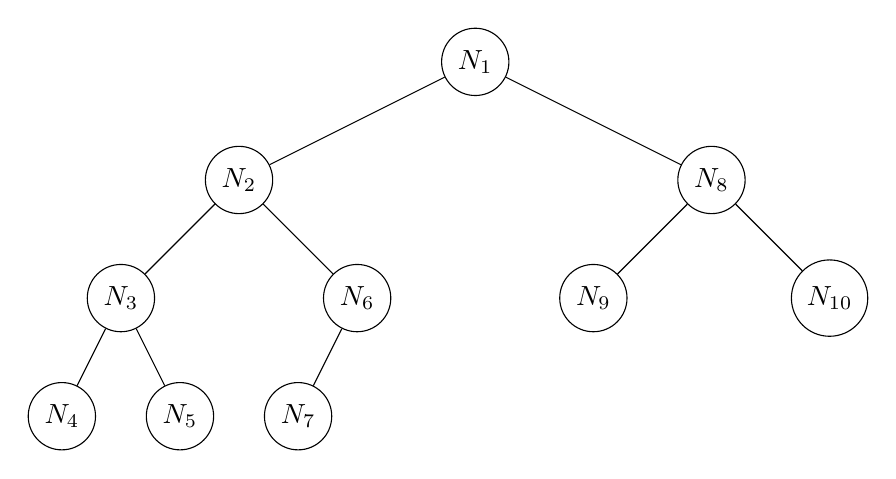
\begin{tikzpicture}
  [level 1/.style={sibling distance=60mm},
  level 2/.style={sibling distance=30mm},
  level 3/.style={sibling distance=15mm}]
\node [circle, draw] {$N_1$}
child {
  node [circle, draw] {$N_2$}
  child {
    node [circle, draw] {$N_3$}
    child {
      node [circle, draw] {$N_4$}
    }
    child {
      node [circle, draw] {$N_5$}
    }
  }
  child {
    node [circle, draw] {$N_6$}
    child {
      node [circle, draw] {$N_7$}
    }
    child {
      node {} edge from parent [draw=none]
    }
  }
}
child {
  node [circle, draw] {$N_8$}
  child {
    node [circle, draw] {$N_9$}
  }
  child {
    node [circle, draw] {$N_{10}$}
  }
};
\end{tikzpicture}
\end{center}

\begin{problemparts}
\problempart \points{1} $\attribix{N_4}{\gamma}$ is
\begin{enumerate}
  \item 0
  \item 1
  \item 2
  \item the key at $N_4$ 
\end{enumerate}
\solution {
  1. A leaf's subtree has exactly one node.
}

\problempart \points{1} $\attribix{N_3}{\gamma}$ is
\begin{enumerate}
  \item 1
  \item 2
  \item 3
  \item the key at $N_4$
  \item the key at $N_5$
  \item the sum of keys at $N_3 \dots N_5$
\end{enumerate}
\solution {
  3
}

\problempart \points{1} $\attribix{N_2}{\gamma}$ is
\begin{enumerate}
  \item 2
  \item 3
  \item 4
  \item 6
  \item the key at $N_4$
  \item the key at $N_7$
  \item the sum of keys at $N_3 \dots N_5$
\end{enumerate}
\solution {
  6
}

\problempart \points{1} $\attribix{N_1}{\gamma}$ is
\begin{enumerate}
  \item 3
  \item 6
  \item 7
  \item 10
  \item the key at $N_4$
  \item the key at $N_{10}$
  \item the sum of keys at $N_1 \dots N_{10}$
\end{enumerate}
\solution {
  10. The questions should show the pattern for computing $\attribix{node}{\gamma}$,
  which is
\begin{eqnarray*}
\attribix{node}{\gamma} &=& 1 + \gamma(\id{left}) + \gamma(\id{right}) \\
\attribix{\const{nil}}{\gamma} &=& 0
\end{eqnarray*}
}

\problempart \points{6} Which of the following functions need to be modified to
update $\gamma$? If a function does not apply to the tree for the range index,
it doesn't need to be modified. (True / False)
\begin{enumerate}
  \item \proc{insert}
  \item \proc{delete}
  \item \proc{rotate-left}
  \item \proc{rotate-right}
  \item \proc{rebalance}
  \item \proc{heapify}
\end{enumerate}
\solution {
  \proc{rotate-left}, \proc{rotate-right}, and \proc{rebalance}
  
  $\gamma$ needs to be updated in the same situations where a node's height is
  updated. The AVL methods that call \proc{update-height} are
  \proc{rotate-left}, \proc{rotate-right}, and \proc{rebalance}. \proc{insert}
  and \proc{delete} rely on the rotation methods to update the height.
}

\problempart \points{1} What is the running time of a $\proc{Count}()$
implementation based on $\proc{Rank}()$?
\begin{enumerate}
  \item $O(1)$
  \item $O(\log(\log N))$
  \item $O(\log N)$
  \item $O(\log^2 N)$
  \item $O(\sqrt{N})$
\end{enumerate}
\solution {
  $O(\log N)$, which can be achieved by the algorithm below.

  \begin{codebox}
  \Procname{$\proc{Rank}(\id{tree}, \id{k})$}
  \li $\id{r} \gets 0$
  \li $\id{node} \gets \attribii{tree}{root}$
  \li \While $\id{node} \neq \const{nil}$
  \li \Do
        \If $\id{k} < \attribii{node}{key}$
  \li   \Then
          $\id{node} \gets \attribii{node}{left}$
  \li   \Else
  \li     \If $\attribii{node}{left} \neq \const{nil}$
  \li     \Then
            $\id{r} \gets \id{r} + 1 + \attribii{\attribii{node}{left}}{\gamma}$
  \li     \Else
  \li       $\id{r} \gets \id{r} + 1$
          \End
  \li     \If $\attribii{node}{key} \isequal \id{k}$
  \li     \Then
            \Return $\id{r}$
          \End
  \li     $\id{node} \gets \attribii{node}{right}$
        \End
      \End
  \li \Return $\id{r}$
  \end{codebox}
  
  The structure is very similar to that of \proc{Find} -- in the worst case,
  \proc{Rank} visits all the nodes on a path from the root to a leaf, and does a
  constant amount of computation at each node on the path.
}
\end{problemparts}

After the analytics data is plotted using Pretty Graph\texttrademark{}, the CEO
can hover the mouse cursor over one of the bars, and the graph will show a
tooltip with the information represented by that bar. To support this operation,
the range index needs to support a $\proc{List}(l, h)$ operation that returns
all the keys between $l$ and $h$ as quickly as possible.

$\proc{List}(l, h)$ cannot be sub-linear in the worst case, because
$\proc{List}(-\infty, +\infty)$ must return all the keys in the index, which
takes $\Omega(n)$ time. However, if $\proc{List}$ only has to return a few
elements, we would like it to run in sub-linear time. We formalize this by
stating that $\proc{List}$'s running time should be $T(N) + \Theta(L)$, where
$L$ is the length of the list of keys output by $\proc{List}$, and $T(N)$ is
sub-linear.

Inspiration (or your 6.006 TA) strikes again, and you find yourself with
the following pseudocode for $\proc{List}$.

\begin{codebox}
\Procname{$\proc{List}(\id{tree}, \id{l}, \id{h})$}
\li $\id{lca} \gets \proc{LCA}(\id{tree}, \id{l}, \id{h})$
\li $\id{result} \gets []$
\li $\proc{Node-List}(lca, \id{l}, \id{h}, \id{result})$
    \label{li:list-node-list}
\li \Return \id{result}
\end{codebox}

\begin{codebox}
\Procname{$\proc{Node-List}(\id{node}, \id{l}, \id{h}, \id{result})$}
\li \If $\id{node} \isequal \const{nil}$
\li   \Then
        \Return  \label{li:node-list-ret}
    \End
\li \If $l \le \attribii{node}{key}$ and $\attribii{node}{key} \le h$ 
\li   \Then
        $\proc{Add-Key}(\id{result}, \attribii{node}{key})$
    \End
\li \If $\attribii{node}{key} \ge l$
    \label{li:node-list-prune-l}
\li   \Then
        $\proc{Node-List}(\attribii{node}{left}, \id{l}, \id{h}, \id{result})$
    \End
\li \If $\attribii{node}{key} \le h$
    \label{li:node-list-prune-r}
\li   \Then
        $\proc{Node-List}(\attribii{node}{right}, \id{l}, \id{h}, \id{result})$
    \End
\end{codebox}

\begin{codebox}
\Procname{$\proc{LCA}(\id{tree}, \id{l}, \id{h})$}
\li $\id{node} \gets \attribii{tree}{root}$
\li \kw{until} $node \isequal \const{nil}$ or
           ($l \le \attribii{node}{key}$ and $h \ge \attribii{node}{key}$)
    \label{li:lca-loop}
\li    \Do
          \If $l < \attribii{node}{key}$
          \label{li:lca-branch-direction}
\li         \Then
              $\id{node} \gets \attribii{node}{left}$
              \label{li:lca-go-left}
\li         \Else
\li           $\id{node} \gets \attribii{node}{right}$
              \label{li:lca-go-right}
          \End
    \End
\li \Return \id{node}
\end{codebox}

\begin{problemparts}

\problempart \points{1} $\proc{LCA}$ most likely means
\begin{enumerate}
  \item last common ancestor
  \item lowest common ancestor
  \item low cost airline
  \item life cycle assessment
  \item logic cell array
\end{enumerate}
\solution {
  Visiting the Wikipedia page for LCA shows that ``lowest common ancestor'' is
  the only computer science-related interpretation of LCA.
}
  
\problempart \points{1} The running time of $\proc{LCA}(l, h)$ for the trees
used by the range index is
\begin{enumerate}
  \item $O(1)$
  \item $O(\log(\log N))$
  \item $O(\log N)$
  \item $O(\log^2 N)$
  \item $O(\sqrt{N})$
\end{enumerate}
\solution {
  $O(\log N)$, the height of the tree.
}

\problempart \points{1} Assuming that $\proc{Add-Key}$ runs in $O(1)$ time,
and that $\proc{List}$ returns a list of $L$ keys, the running time of the
$\proc{Node-List}$ call at line \ref{li:list-node-list} of $\proc{List}$ is
\begin{enumerate}
  \item $O(1)$
  \item $O(\log(\log N))$
  \item $O(\log N)$
  \item $O(\log^2 N)$
  \item $O(\sqrt{N})$
  \item $O(1) + O(L)$
  \item $O(\log(\log N)) + O(L)$
  \item $O(\log N) + O(L)$
  \item $O(\log^2 N) + O(L)$
  \item $O(\sqrt{N}) + O(L)$
\end{enumerate}
\solution {
  $O(\log N) + O(L)$.
  
  The \proc{Node-List} call at line \ref{li:list-node-list} performs a pre-order
  traversal starting at the least common ancestor of the nodes containing keys
  $l$ and $h$. If the keys $l$ and/or $h$ are not in the BST, we use the
  positions of imaginary nodes that would be created by inserting $l$ and/or $h$
  using the BST insertion algorithm (no re-balancing).
  
  The traversal ignores some sub-trees. Line \ref{li:node-list-prune-l} prunes
  the left sub-tree of any node whose key is $\le l$ because, by the BST
  invariant, the keys of all the nodes in the sub-tree will be smaller than
  $\attribii{node}{key}$, which is $\le l$. In a symmetric fashion, line
  $\label{li:node-list-prune-r}$ prunes sub-trees where all the nodes' keys are
  guaranteed to be greater than $h$.
  
  \proc{Node-List} spends $O(1)$ time for each node it visits, so the total
  running time is $O(V)$, where $V$ is the number of visited nodes. We split up
  $V = L + X$, where $L$ is the number of nodes returned from \proc{List}, and
  $X$ is the number of nodes that are visited, but not output (extra nodes, or
  overhead). We argue that $X = O(h)$, where $h$ is the height of the BST.
  Because the BST is an AVL, we use $h = O(\log N)$ to conclude that the total
  running time of the \proc{Node-List} call in \proc{List} is $O(\log(N) + L)$.
  
  We'll sketch a proof that the extra nodes in the left sub-tree of the LCA node
  are all on the path from the LCA to the $l$ node. A symmetric proof covers the
  right sub-tree of the LCA node. The proof refers to the tree below.
  
  \begin{center}
  \hspace*{-25mm}
  \begin{tikzpicture}
    [level 1/.style={sibling distance=140mm, level distance=10mm},
    level 2/.style={sibling distance=50mm, level distance=10mm},
    level 3/.style={sibling distance=30mm, level distance=10mm}]
  \node [circle, draw] {LCA}
  child {
    node {$\vdots$}
    child {
      node {} edge from parent [draw=none]
    }
    child {
      node [circle, draw] {$x$}
      child {
        node [regular polygon,regular polygon sides=3, draw] {$x_L$}
      }
      child {
        node [circle, draw] {$y$}
        child {
          node {$\vdots$}
          child {
            node [circle, draw] {$l$}
          }
        }
        child {
          node [regular polygon,regular polygon sides=3, draw] {$y_R$}
        }
      }
    }
  }
  child {
    node {$\vdots$}
    child {
      node [circle, draw] {$h$}
    }
  };
  \end{tikzpicture}
  \end{center}
  
  Every node on the path from the LCA node to the $l$ node falls under one of
  the following two cases.
  \begin{itemize}
    \item The node $l$ belongs to the node's right sub-tree. Let $x$ be the
    node's key, and $x_L$ be the node's left sub-tree. Since the $l$ node is in
    the $x$ node's left sub-tree, it follows that $l > x$ (by theBST
    invariant), so the $x_L$ sub-tree will be pruned by line
    \ref{li:node-list-prune-l} in \proc{Node-List}. So \proc{Node-List} will
    never ``stray'' to the left of the path from the LCA node to the $l$ node.
     
    \item The node $l$ belongs to the node's left sub-tree. Let $y$ be the
    node's key, and $y_R$ be the node's right sub-tree. Since the $l$ node is in
    the $x$ node's right sub-tree, it follows that $l < y$ (by the BST's
    invariant). Every node in $y_R$ will have a key greater than $y$ (BST
    invariant), so all the keys in $y_R$ are greater than $l$. Furthermore,
    because $y_R$ is in LCA's left sub-tree, all the keys in $y_R$ are smaller
    than the key in LCA, which is $\le h$. It follows that all the nodes in
    $y_R$ belong to the $(l, h]$ interval, and their keys will be returned from
    \proc{Node-List}. So, whenever \proc{Node-List} ``strays'' to the right of
    the path from the LCA node to the $l$ node, it will output all the nodes it
    encounters.
  \end{itemize}
  
  The two cases above show that all the extra nodes (visited but not added to
  the result) in the LCA node's left sub-tree are on the path from LCA to $l$,
  which means $X = O(h)$. A symmetric proof can be used to show that all the
  extra nodes in the LCA node's right sub-tree are on the path from LCA to $h$.
}

\problempart \points{1} Assuming that $\proc{Add-Key}$ runs in $O(1)$ time,
and that $\proc{List}$ returns a list of $L$ keys, the running time of
$\proc{List}$ is
\begin{enumerate}
  \item $O(1)$
  \item $O(\log(\log N))$
  \item $O(\log N)$
  \item $O(\log^2 N)$
  \item $O(\sqrt{N})$
  \item $O(1) + O(L)$
  \item $O(\log(\log N)) + O(L)$
  \item $O(\log N) + O(L)$
  \item $O(\log^2 N) + O(L)$
  \item $O(\sqrt{N}) + O(L)$
\end{enumerate}
\solution {
  $O(\log N) + O(L)$. According to the previous questions, \proc{LCA} takes
  $O(\log N)$ time, and the \proc{Node-List} call takes $O(\log N) + O(L)$ time.
}

\problempart \points{20} Prove that $\proc{LCA}$ is correct.

\solution {
  We will argue that $\proc{LCA}(l, h)$ returns the least-common ancestor,
  defined as the root of the smallest sub-tree that contains both $l$ and $h$.
  If the keys $l$ and/or $h$ are not in the BST, we augment the tree with the
  imaginary nodes that would be created by inserting $l$ and/or $h$ using the
  BST insertion algorithm (no re-balancing).
  
  Based on the definition above, we will prove that \proc{LCA} is correct in two
  stages: first we prove that \proc{LCA} maintains the invariant that $l$ and
  $h$ belong to the sub-tree rooted at \id{node}, then we prove that \proc{LCA}
  returns the root of the smallest sub-tree that contains both $l$ and $h$.
  
  \textbf{\proc{LCA} maintains the invariant that $l$ and $h$ belong to the
  sub-tree rooted at \id{node}}. \id{node} starts out at the tree's root, so the
  invariant starts out to be true at line \ref{li:lca-loop}. The loop continues
  as long as both $l$ and $h$ are smaller than \id{node}'s key, or $l$ and $h$
  are both bigger than \id{node}'s key. If $l$ and $h$ are smaller, then the
  condition on line \ref{li:lca-branch-direction} will be true, so both $l$ and
  $h$ are in \id{node}'s left sub-tree, by the BST invariant, so line
  \ref{li:lca-go-left} preserves the invariant. Similarly, if $l$ and $h$ are
  larger, they're both in \id{node}'s right sub-tree, so line
  \ref{li:lca-go-right} preserves the invariant.
  
  \textbf{\proc{LCA} returns the root of the smallest sub-tree that contains
  both $l$ and $h$}. Proof by contradiction:
  
  Let $r$ be the key of the node returned by \proc{LCA}, and $c$ be the key of
  the node that is the correct answer. By the invariant above, $l$ and $h$ are
  in the sub-tree rooted at the $r$ node, so the $c$ node is in the sub-tree
  rooted at $r$.
  
  If $c$ is in the $r$ node's left sub-tree, it follows that $c < r$. Since $l$
  and $h$ are in the sub-tree rooted at the $c$ node, they are in $r$'s left
  sub-tree, so $l < r$ and $h < r$ by the BST invariant. But in that case, the
  condition on line \ref{li:lca-loop} will be true when id{node} is the $r$
  node, so the $r$ node should not be returned from \proc{LCA}. Contradiction.
  
  The case where $c$ is in the $r$ node's right sub-tree is symmetrical, as both
  $l$ and $h$ will be in $r$'s sub-tree and $l > r$, $h > r$.
}
\end{problemparts}

\newpage

\problem \points{55} \textbf{Digital Circuit Layout}

Your AMDtel internship is off to a great start! The optimized circuit simulator
cemented your reputation as an algorithms whiz. Your manager capitalized on your
success, and promised to deliver the Bullfield chip a few months ahead of
schedule. Thanks to your simulator optimizations, the engineers have finished
the logic-level design, and are currently working on laying out the gates on the
chip. Unfortunately, the software that verifies the layout is taking too long to
run on the preliminary Bullfield layouts, and this is making the engineers slow
and unhappy. Your manager is confident in your abilities to speed it up, and
promised that you'll ``do your magic'' again, in ``one week, two weeks tops''.

A chip consists of logic gates, whose input and output terminals are connected
by wires (very thin conductive traces on the silicon substrate). AMDtel's
high-yield manufacturing process only allows for horizontal or vertical wires.
Wires must not cross each other, so that the circuit will function according to
its specification. This constraint is checked by the software tool that you
will optimize. The topologies required by complex circuits are accomplished by
having dozens of layers of wires that do not touch each other, and the tool
works on one layer at a time.

\begin{problemparts}
\problempart \points{1} Run the code under the python profiler with the command
below, and identify the method that takes up most of the CPU time. If two
methods have similar CPU usage times, ignore the simpler one.

\texttt{python -m cProfile -s time circuit2.py < tests/10grid\_s.in}

\textit{Warning:} the command above can take 15-60 minutes to complete, and
bring the CPU usage to 100\% on one of your cores. Plan accordingly. If
you have installed PyPy successfully, you can replace \texttt{python} with
\texttt{pypy} in the command above for a roughly 2x speed improvement. 

What is the name of the method with the highest CPU usage?
\solution {
  The first line in the profiler output identifies \texttt{intersects} as the
  method with the largest CPU usage.
}

\problempart \points{1} How many times is the method called?
\solution {
  The first line in the profiler output indicates that \texttt{intersects} is
  called 187590314 times.
}
\end{problemparts}

The method that has the performance bottleneck is called from the
\texttt{CrossVerifier} class. Upon reading the class, it seems that the original
author was planning to implement a \textit{sweep-line} algorithm, but
couldn't figure out the details, and bailed and implemented an inefficient
method at the last minute. Fortunately, most of the infrastructure for a fast
sweep-line algorithm is still in place. Furthermore, you notice that the
source code contains a trace of the working sweep-line algorithm, in the
\texttt{good\_trace.jsonp} file.

Sweep-line algorithms are popular in computational geometry. Conceptually,
such an algorithm sweeps a vertical line left to right over the plane containing
the input data, and performs operations when the line ``hits'' point of interest
in the input. This is implemented by generating an array containing all the
points of interest, and then sorting them according to their position along the
horizontal axis ($x$ coordinate).

Read the source for \texttt{CrossVerifier} to get a feel for how the sweep-line
infrastructure is supposed to work, and look at the good trace in the
visualizer that we have provided for you. To see the good trace, copy
\texttt{good\_trace.jsonp} to \texttt{trace.jsonp}

\texttt{cp good\_trace.jsonp trace.jsonp}

On Windows, use the following command instead.

\texttt{copy good\_trace.jsonp trace.jsonp}

Then use Google Chrome to open \texttt{visualizer/bin/visualizer.html}

The questions below refer to the fast sweep-line algorithm shown in
\texttt{good\_trace.jsonp}, not to the slow algorithm hacked together in
\texttt{circuit2.py}.

\begin{problemparts}
\problempart \points{5} The $x$ coordinates of points of interest in the input
are (True / False)
\begin{enumerate}
  \item the $x$ coordinates of the left endpoints of horizontal wires
  \item the $x$ coordinates of the right endpoints of horizontal wires
  \item the $x$ coordinates of midpoints of horizontal wires
  \item the $x$ coordinates where horizontal wires cross vertical wires
  \item the $x$ coordinates of vertical wires
\end{enumerate}
\solution {
  The $x$ coordinates of both endpoints of horizontal wires, and of vertical
  wires. The algoritm doesn't handle wire midpoints specially. Crossing points
  cannot possibly be points of interest, because they are the algorithm's
  output, not input.
}

\problempart \points{1} When the sweep line hits the $x$ coordinate of the left
endpoint of a horizontal wire
\begin{enumerate}
  \item the wire is added to the range index
  \item the wire is removed from the range index
  \item a range index query is performed
  \item nothing happens
\end{enumerate}
\solution {
  The wire is added to the range index when the sweep line hits the $x$
  coordinate of the left endpoint.
}

\problempart \points{1} When the sweep line hits the $x$ coordinate of the right
endpoint of a horizontal wire
\begin{enumerate}
  \item the wire is added to the range index
  \item the wire is removed from the range index
  \item a range index query is performed
  \item nothing happens
\end{enumerate}
\solution {
  The wire is removed from the range index when the sweep line hits the X
  coordinate of the right endpoint.
}

\problempart \points{1} When the sweep line hits the $x$ coordinate of the
midpoint of a horizontal wire
\begin{enumerate}
  \item the wire is added to the range index
  \item the wire is removed from the range index
  \item a range index query is performed
  \item nothing happens
\end{enumerate}
\solution {
  Nothing happens.
}

\problempart \points{1} When the sweep line hits the $x$ coordinate of a 
vertical wire
\begin{enumerate}
  \item the wire is added to the range index
  \item the wire is removed from the range index
  \item a range index query is performed
  \item nothing happens
\end{enumerate}
\solution {
  A range index is performed.
}

\problempart \points{1} What is a good invariant for the sweep-line algorithm?

\begin{enumerate}
  \item the range index holds all the horizontal wires to the left of the
  sweep line
  \item the range index holds all the horizontal wires ``stabbed'' by the
  sweep line
  \item the range index holds all the horizontal wires to the right of the
  sweep line
  \item the range index holds all the wires to the left of the sweep line
  \item the range index holds all the wires to the right of the sweep line
\end{enumerate}
\solution {
  The invariant for the sweep-line algorithm is that the range index holds all
  the horizontal wires ``stabbed'' by the sweep line.
}

\problempart \points{1} When a wire is added to the range index, what is its
corresponding key?

\begin{enumerate}
  \item the $x$ coordinate of the wire's midpoint
  \item the $y$ coordinate of the wire's midpoint
  \item the segment's length
  \item the $x$ coordinate of the point of interest that will remove the wire
  from the index
\end{enumerate}
\solution {
  The only correct answer is ``the Y coordinate of the wire's midpoint''.
  Only horizontal wires are added to the range index, and all their points have
  the same Y coordinate.
}
\end{problemparts}

Modify \texttt{CrossVerifier} in \texttt{circuit2.py} to implement the
sweep-line algorithm discussed above. If you maintain the current code
structure, you'll be able to use our visualizer to debug your implementation. To
use our visualizer, first produce a trace.

\texttt{TRACE=jsonp python circuit2.py < tests/5logo.in > trace.jsonp}

On Windows, run the following command instead.

\texttt{circuit2\_jsonp.bat < tests/5logo.in > trace.jsonp}

Then use Google Chrome to open \texttt{visualizer/bin/visualizer.html}

\begin{problemparts}
\problempart \points{1} Run your modified code under the python profiler again,
using the same test case as before, and identify the method that takes up the
most CPU time.

What is the name of the method with the highest CPU usage? If two methods have
similar CPU usage times, ignore the simpler one.
\solution {
  The first line in the profiler output identifies \texttt{count} as the
  method with the highest CPU usage.
}

\problempart \points{1} How many times is the method called?
\solution {
  The first line in the profiler output indicates that \texttt{count} is
  called 20000 times.
}

\problempart \points{40} Modify \texttt{circuit2.py} to implement a data
structure that has better asymptotic running time for the operation above. Keep
in mind that the tool has two usage scenarios:

\begin{itemize}
  \item Every time an engineer submits a change to one of the Bullhorn wire
  layers, the tool must analyze the layer and report the number of wire
  crossings. In this late stage of the project, the version control system will
  automatically reject the engineer's change if it causes the number of wire
  crossings to go up over the previous version.
  \item Engineers working on the wiring want to see the pairs of wires that
  intersect, so they know where to focus ther efforts. To activate this detailed
  output, run the tool using the following command.

  \texttt{TRACE=list python circuit2.py < tests/6list\_logo.in}
  
  On Windows, run the following command instead.
  
  \texttt{circuit2\_list.bat < tests/6list\_logo.in}
\end{itemize}

When your code passes all tests, and runs reasonably fast (the tests should
complete in less than 60 seconds on any reasonably recent computer), upload your
modified \texttt{circuit.py} to the course submission site.

\solution {
  The solution archive on the course Web site contains the staff's solution and
  secret test cases.
}
\end{problemparts}

\end{problems}
\end{document}
